\documentclass{beamer}
\usepackage{graphicx}
\usepackage{caption}
%\usepackage{subcaption}
\usepackage{color}
\usepackage{amssymb}
\usepackage{xcolor}
\usepackage{wrapfig}
\usepackage{amsmath}
\usepackage[
backend=bibtex,
sorting=none,
style=authoryear
]{biblatex}
\addbibresource{bibliography.bib}

\defbibenvironment{nolabelbib}
  {\list
     {}
     {\setlength{\leftmargin}{\bibhang}%
      \setlength{\itemindent}{-\leftmargin}%
      \setlength{\itemsep}{\bibitemsep}%
      \setlength{\parsep}{\bibparsep}}}
  {\endlist}
  {\item}

\setbeamertemplate{navigation symbols}{}
\usetheme{CambridgeUS}
\usecolortheme{beaver} 

\beamersetuncovermixins{\opaqueness<1>{25}}{\opaqueness<2->{15}}

%\pgfdeclareimage[height=2cm]{i4}{pic/acat.pdf}


%\author[Dzmitry Makatun]{\textbf{Dzmitry~Makatun} \inst{1} $^{,}$ \inst{2}}

\author[Dzmitry Makatun]{\textbf{Dzmitry~Makatun} \inst{1} \inst{3} \and J\'er\^ome~Lauret\inst{2}\\ \and Michal~\v{S}umbera \inst{1} \and Hana~Rudov\'a \inst{4}}
\title[Distributed data production planning]{Model for planning of distributed data production} 
\institute [NPI ASCR]
{ 
  \inst{1}%
  Nuclear Physics Institute, Academy of Sciences, Czech Republic
  \pgfdeclareimage[height=2cm]{i1}{pic/ujf.pdf}   
  \and
  \inst{2}%
  Brookhaven National Laboratory, USA
  \pgfdeclareimage[height=2cm]{i2}{pic/STAR.pdf}
  \and
  \inst{3}
Czech Technical University in Prague, Czech Republic  
\pgfdeclareimage[height=2cm]{i3}{pic/ctu.pdf} 
\and
\inst{4}
Faculty of Informatics, Masaryk University, Czech Republic
\pgfdeclareimage[height=2cm]{i6}{pic/fjfi.pdf}
\pgfdeclareimage[height=2cm]{i8}{pic/doe.pdf}
 
\vspace{-4mm}   
  \pgfuseimage{i1}
  \pgfuseimage{i2}
  \pgfuseimage{i3}
  %\pgfuseimage{i4}
  %\pgfuseimage{i5}
  %\pgfuseimage{i6}
  %\pgfuseimage{i8}

  \vspace{-7mm}
\begin{center}
d.i.makatun@gmail.com
\end{center}
\vspace{-5mm}
  }
\begin{document}
\date{27.08.2015} 

\begin{frame}
\titlepage
\end{frame}

\begin{frame}\frametitle{Outline}
\tableofcontents
\end{frame}

\section{Introduction}
\subsection{Data processing in High Energy Nuclear Physics (HENP)}

\begin{frame}\frametitle{Computations in HENP: What do we compute?}
\begin{figure}
\begin{center}
%\vspace{-1 cm}
\includegraphics[ height=0.4\textheight]{pic/rhic.jpg}
\hspace{0.5cm}
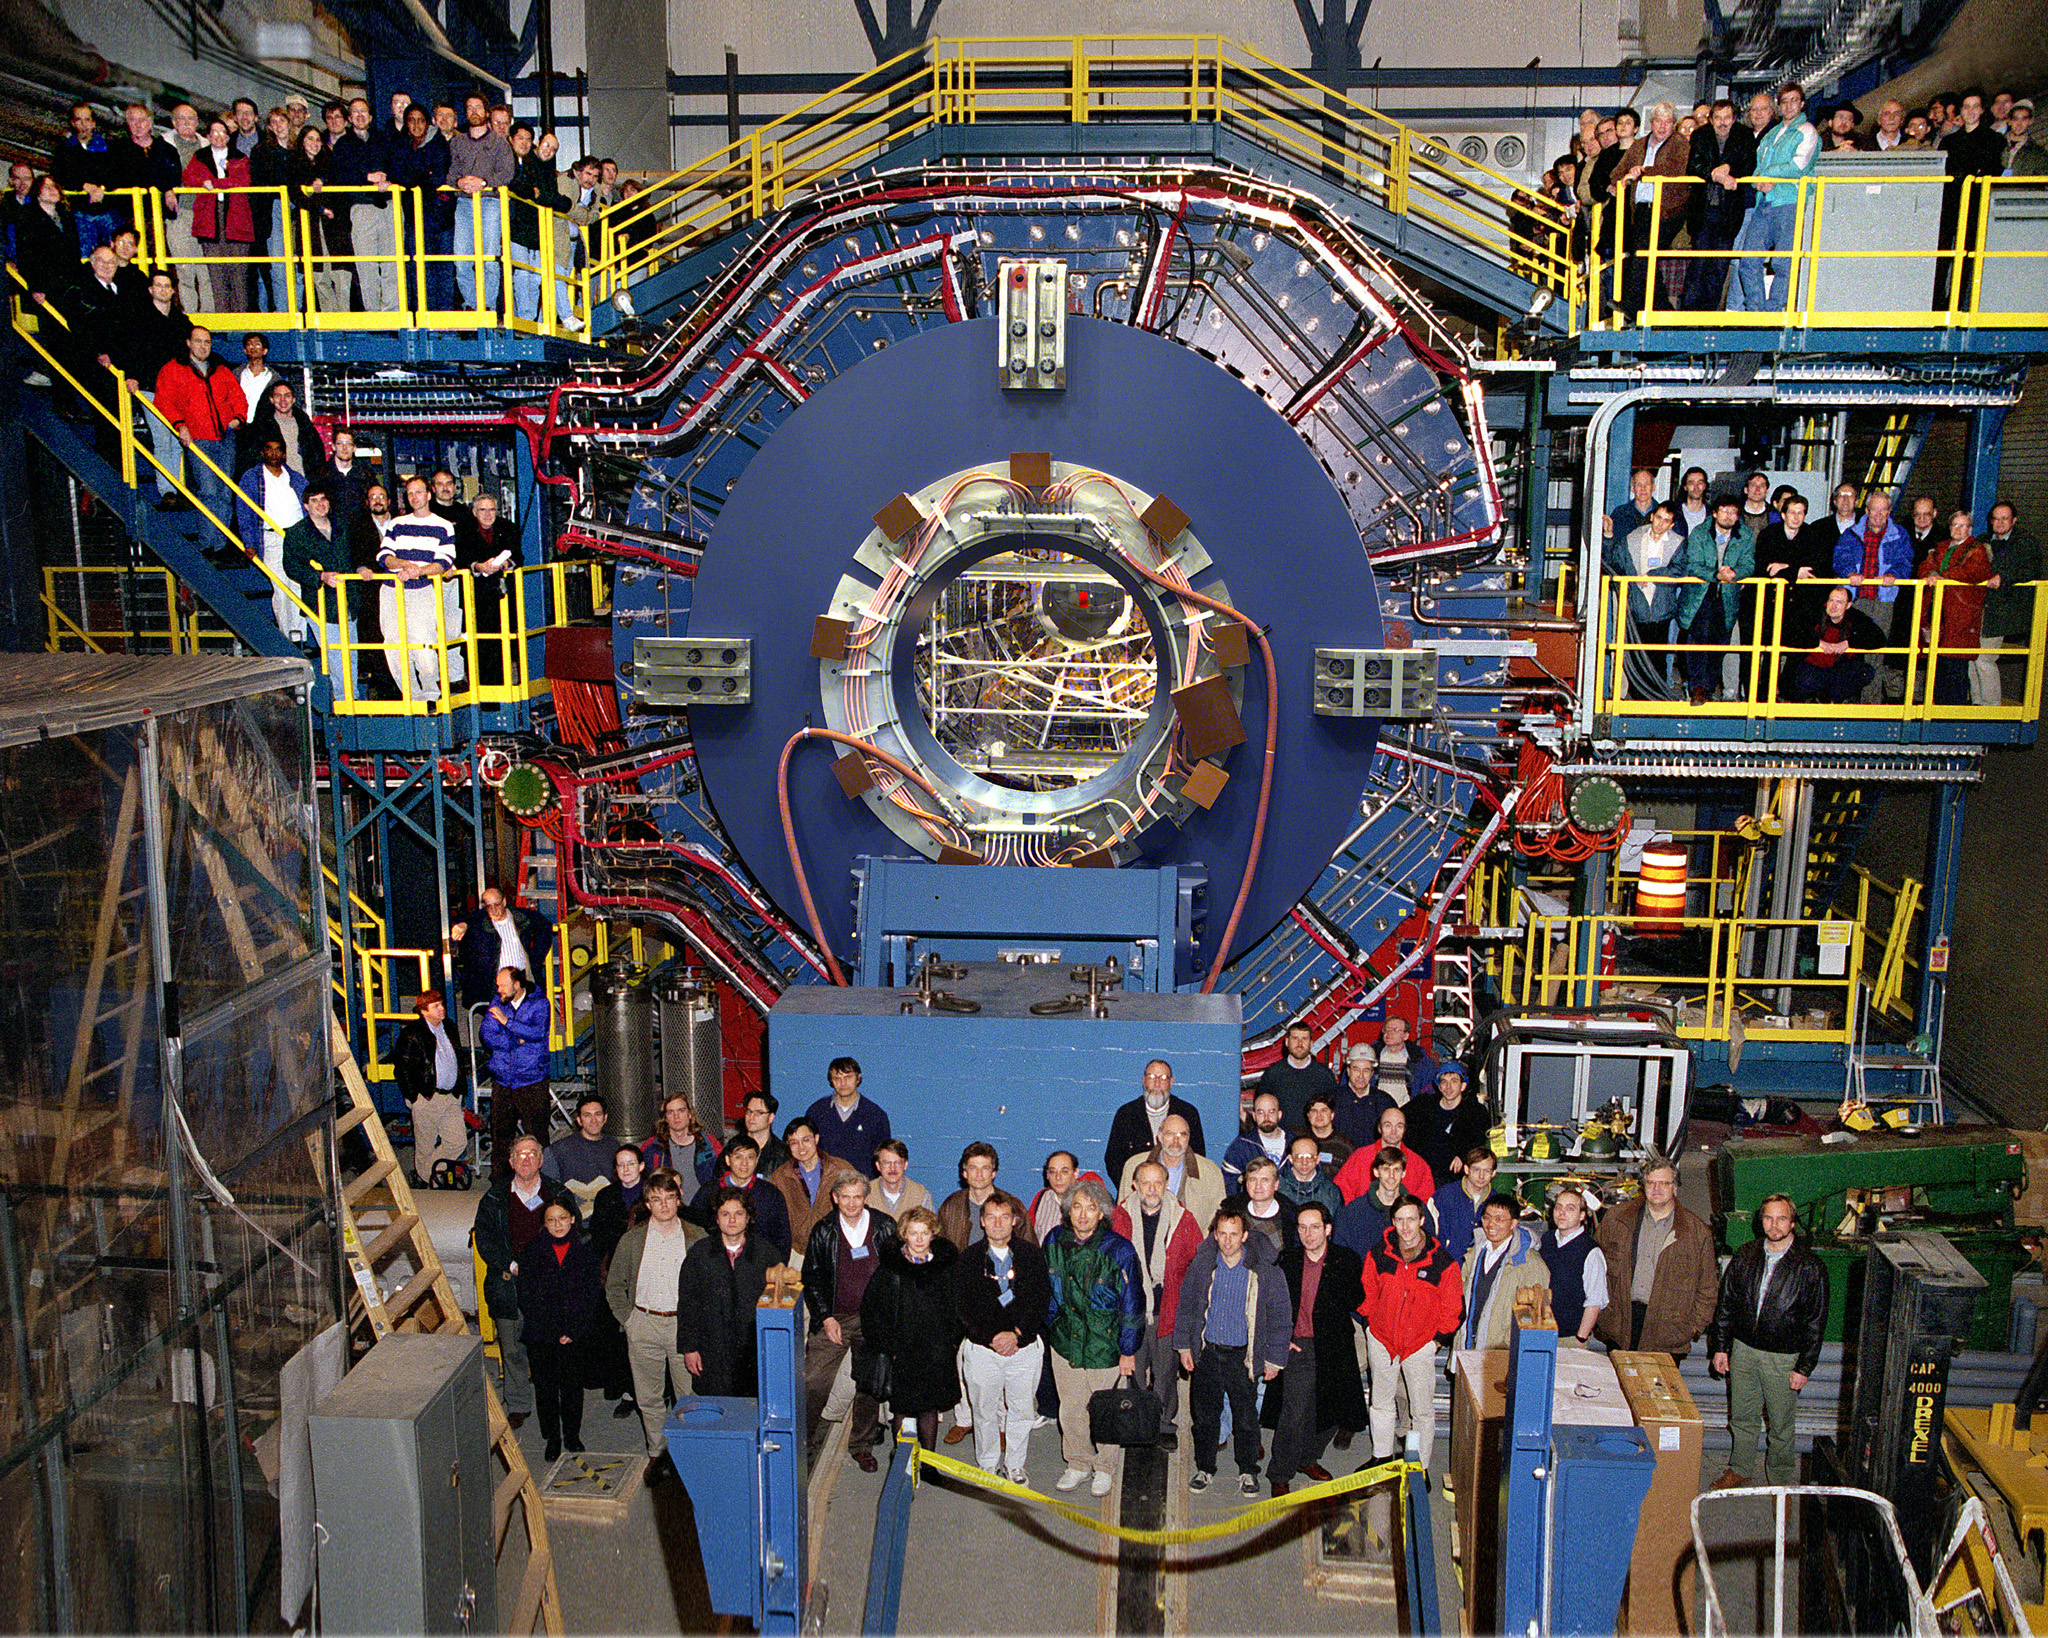
\includegraphics[ height=0.4\textheight]{pic/star.jpg}
\end{center}
\end{figure}
\vspace{-1 cm}
\begin{block}{}
		\begin{itemize}
			\item Brookhaven National Laboratory (\textbf{BNL}) Long Island, NY, USA.
			\item Relativistic Heavy Ion Collider (\textbf{RHIC}). A quark-gluon plasma is created in heavy ion collisions to study the form of matter that existed shortly after the Big Bang.
			\item Solenoid Tracker at RHIC (\textbf{STAR}). Collisions occur millions of times per second. Events of size 200 MB are processed at rates up to 100~Hz. Raw data output rate is $\sim$ \textcolor{red} {30 MB/sec}.
		\end{itemize}
 	\end{block}
\end{frame}

\begin{frame}\frametitle{Computations in HENP: How do we compute?}
\begin{columns}[c]
  \column{.7\textwidth}
    \begin{block}{Stages}
      \begin{enumerate}      
        \item \textbf{Data Production:} The raw output data is processed to reconstruct events ($\sim$ ones).\\
        \item \textbf{User Analysis:} Reconstructed events are analyzed by scientists (many times).\\
      \end{enumerate}
 	\end{block}
 	
    \begin{block}{At RHIC Computing Facility (RCF): } 	
      \begin{itemize}
	    \item All the data (raw, reconstructed and analysis output) permanently stored on tape.
	    \item $\sim$ 31 PB of data.
        \item $\sim$ 12 000 jobs running simultaneously.\\
      \end{itemize}
    \end{block}

 \textbf{Growing usage of remote computing facilities.}

  \column{.3\textwidth}
  \begin{figure}
    \begin{center}
      \includegraphics[ height=0.35\textheight]{pic/nersc.jpg}
      
    \end{center}
  \end{figure} 
    \begin{figure}
    \begin{center}
      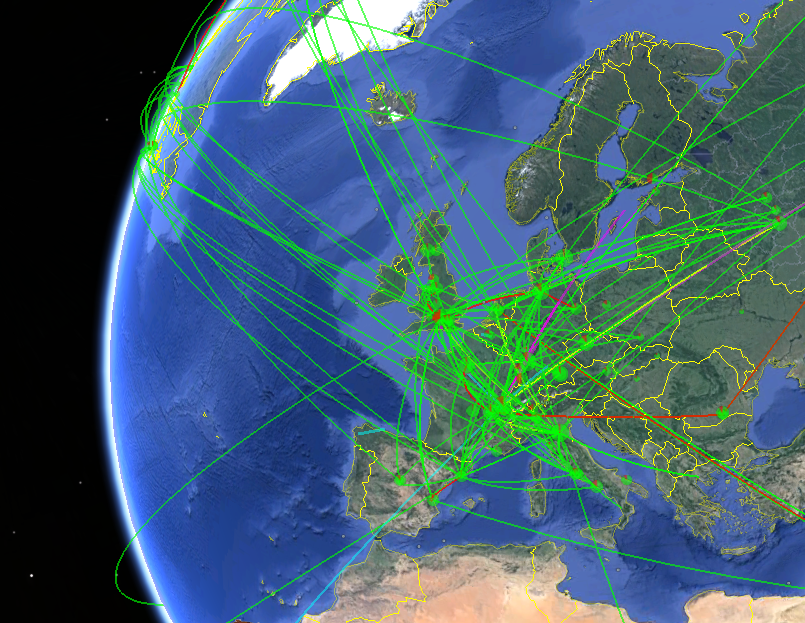
\includegraphics[ height=0.3\textheight]{pic/grid-net.png}
    \end{center}
  \end{figure} 	
\end{columns}
\end{frame}

\begin{frame}\frametitle{Data production vs User analysis (in Grid)}
\begin{columns}[c]
\column{.45\textwidth}
\begin{block}{}
Grid = network of computational servers
\end{block}

\begin{block}{Data production}
  \begin{itemize}
    \item Single central storage
    \item 1 job per file
    \item 1 CPU per job
    \item Input size $\approx$ Output size 
  \end{itemize}
  Lack of dedicated solution
\end{block}

\column{.45\textwidth}
\begin{block}{User analysis}
  \begin{itemize}
    \item Distributed storage	
    \item Data replication
	\item Data processed by multiple jobs
	\item Output size is negligible compared to input size
  \end{itemize}
  Most load-balancing tools consider similar scenario \textcolor{black}{[\cite{Globus_scheduler}]}
\end{block}

\end{columns}


\begin{block}{}
In our research we \textbf{focus on data production} in HENP.
\end{block}
\end{frame}


\begin{frame}\frametitle{Data production: simplified view }
 	\begin{columns}[c] % the "c" option specifies center vertical alignment
    \column{.6\textwidth} % column designated by a command 	
    \begin{footnotesize}
    \vspace{-11mm}
	\begin{block}{Planning remote site usage}
		\begin{itemize}
		\item Input data is located at BNL.
		\item Computational resources are available at BNL and several remote sites.
		\item Output file has to be transferred back to BNL.
		\item \textbf{How should we distribute a given set of files between sites to complete the processing faster?}
		\end{itemize}
 	\end{block} 	
 	
 	\begin{block}{Current solutions} 	
		\begin{itemize}
		  \item Pull a job to free CPU (\textcolor{red}{cons:} I/O overhead)
		  \item Adjust the load manually (\textcolor{red}{cons:} not scalable)
		\end{itemize}
	This should be optimized and automated.
 	\end{block}  	     

 	\end{footnotesize}
 	\column{.4\textwidth}
 		\vspace{-5mm}
		\begin{figure}   
				\includegraphics[trim = 25mm 10mm 0mm 30mm, clip, width=1.2\textwidth]{pic/Data_production_schema2.pdf}
		\end{figure} 	 	
 	\end{columns}
\end{frame}

\begin{frame}\frametitle{Data production: detailed view}
 	\begin{columns}[c] % the "c" option specifies center vertical alignment
    \column{.6\textwidth} % column designated by a command 	
    \begin{footnotesize}
    \vspace{-10mm}
	\begin{block}{New dimensions of the problem}	
		\begin{itemize}		
			\item Several possible data sources
			\item Real network topology: shared links, \textbf{links between remote sites}
			\item Limited storage at sites
			\item \textbf{Which file source to select?}
			\item \textbf{Which transfer path?}

		\end{itemize}
 	\end{block}
		\begin{block}{Example: data-production at ANL  \textcolor{black}{[\cite{Balewski}]}}	
		\begin{itemize}
			\item ANL: many CPU's, but slow connection and small disk space
			\item NERSC: fast connection, large disk
			\item Approach: Feed ANL from both BNL and NERCS sites		

		\end{itemize}
 	\end{block}
 	\end{footnotesize} 
 	\column{.4\textwidth}
		\begin{figure}
			\begin{center}
			    \vspace{-5mm}
				\includegraphics [trim = 25mm 10mm 0mm 30mm, clip, width=1.2\textwidth]{pic/Data_production_schema_ANL2.pdf}
			\end{center}
			\end{figure} 	 	
 	\end{columns}
\end{frame}

\section{Data production planning}
\begin{frame}\frametitle{Data production problem}

\begin{block}{Task}
Create a global scheduler for Grid which will reason about:\\
\hspace{1cm} 1.data~transferring \hspace{1cm} 2.~CPU~allocation\hspace{1cm} 3.~data~storage  
\end{block}
\begin{block}{Rules}  
		\begin{itemize}
			\item None of the resources (network links, data storages and CPUs) are over-saturated at any moment of time.
			\item The jobs are executed  where the data is pre-placed.
			\item Output data is transferred back to the central storage.
			\item No excessive transfers or data replication.
		\end{itemize}
\end{block}
	
\begin{block}{Criteria}
Minimize a makespan for processing of a given dataset 
\end{block}
	
\end{frame}


\subsection{Network flow model}
\begin{frame}\frametitle{Network flow model} 
  \begin{block}{Idea}
    Plan resource load only and then distribute particular jobs accordingly.
  \end{block}

  \begin{block}{Network flow model}
    \begin{itemize}
      \item $\Delta T$ - planning time interval
      \item $Flow$ - amount of data to be transferred
      \item Link capacity - $bandwidth \cdot \Delta T$
    \end{itemize}
  \end{block}    
  Knowing data distribution at the beginning of $\Delta T$,\\
  \textbf{how much data should be transferred over each network link?}
  
    \begin{block}{Sub-problems:}
    \begin{itemize}
      \item Input
      \item Otput
    \end{itemize}
  \end{block}  
  
  Network flow maximization problem can be solved within polynomial time.
\end{frame}

\begin{frame}\frametitle{Input transfer planning}
\textbf{How much data can be transferred during $\Delta T$?}\\
Dummy edges - constraints on  storage and CPUs at each site.
\vspace{-5mm}
\begin{figure}[h]
	\begin{center}
		\includegraphics [trim= 30mm 30mm 30mm 30mm , clip, angle =-90, width=0.7\textwidth]{pic/real_network.pdf}
	\end{center}
	\label{real_network}
\end{figure} 
\vspace{-3mm}
Output flow problem can be formulated similarly.
\end{frame}

\section{Model details}
\begin{frame}\frametitle{Model details: input problem illustration}
\begin{figure}[h]
	\begin{center}
		\includegraphics [trim= 30mm 20mm 30mm 30mm , clip, angle =-90, width=0.7\textwidth]{pic/network_general.pdf}
	\end{center}

	\label{network_general}	
\end{figure} 
$c_{0}$ is a central storage, $c_{i}$ are computational nodes (where $i>0$), $l_{j}$ are network links, $d_{i}$ are dummy edges from computational nodes to the sink $t$, $q_{0}$ is a dummy edge leading from the source $s$ to the $c_{0}$. 
\end{frame}

\begin{frame}<beamer>[noframenumbering]\frametitle{Model details: output problem illustration}
\begin{figure}[h]
	\begin{center}
		\includegraphics [trim= 30mm 20mm 30mm 30mm , clip, angle =-90, width=0.7\textwidth]{pic/network_general_out.pdf}
	\end{center}

	\label{general_out}	
\end{figure}
	$c_{0}$ is a central storage, $c_{i}$ are computational nodes (where $i>0$), $l_{j}$ are network links, $\overline{d}_{i}$ are dummy edges from the source $t$ to computational nodes, $\overline{q}_{0}$ is a dummy edge leading from $c_{0}$ to the sink $s$.
\end{frame}


\begin{frame}<beamer>[noframenumbering]\frametitle{Model details}
\begin{scriptsize}


Input problem:
\begin{equation} 
\label{edge_cap} 
cap(e) = \left\{
\begin{array}{l l} 
b_{j} \cdot \Delta T & \text{if }e = l_{j} \in L \\ w_{i} &
\text{if } e = d_{i} \in D\\ k_{0} & \text{if } e = q_{0} 
\end{array} \right.
\end{equation} 
Output problem:
\begin{equation}
\label{edge_cap_out}
cap(e) = \left\{ 
  \begin{array}{l l}
    b_{j} \cdot \Delta T & \text{if }e = l_{j} \in L \\
    \overline{w}_{i} & \text{if } e = \overline{d}_{i} \in \overline{D}\\
    \overline{k}_{0} & \text{if } e = \overline{q}_{0}
  \end{array} \right.
\end{equation}

Capacities of dummy edges:
\begin{eqnarray}
w_{i} &=&
Disk_{i} - I_{i}^{in} - I_{i}^{out} + \frac{1 - \beta}{\alpha_{i}} \cdot
NCPU_{i} \cdot \Delta T + Del_{i}^{out} \label{w}\\
\overline{w}_{i} &=& I_{i}^{out} + \frac{\beta}{\alpha_{i}} \cdot NCPU_{i} \cdot \Delta T - Min_{i}^{out} \label{sigma}
\end{eqnarray}  
Where $\Delta T$ is a scheduling time interval, $b_{j}$ is a bandwidth of a real network link $j$, $k_{0}$ is the size of input data available at the central storage, $\overline{k}_{0}$ is the free space available at the central storage, $Disk_{i}$ and $NCPU_{i}$ are a storage size and a number of CPUs at the node $i$,  $I_{i}^{in}$ and $I_{i}^{out}$ are the initial size of input and output data at the node, $Del_{i}^{out}$ is the amount of output data that will be transferred out of the node, $Min_{i}^{out}$ is the total size of output files of running jobs. 

\end{scriptsize}
\end{frame}

\begin{frame}\frametitle{Capacities of dummy edges}
\begin{columns}[c]
\column{.45\textwidth}
\begin{block}{Data production of a given dataset}
  \begin{itemize}
    \item Same type of computations
    \item Same type of files 
  \end{itemize}
\end{block}

\begin{block}{Constant parameters}
  \begin{itemize}
    \item $duration \approx \alpha \cdot inputSize $
    \item $ouputSize \approx \beta \cdot  inputSize $ 
  \end{itemize}
\end{block}

\begin{block}{Can predict}
  \begin{itemize}
    \item How fast the data is processed
    \item How much output data is created
  \end{itemize}
\end{block}

\column{.55\textwidth}
\begin{scriptsize}
\vspace{-6mm}
\begin{figure}[h]
	\begin{center}
		\includegraphics [trim= 30mm 50mm 35mm 45mm , clip, width=.95\textwidth]{pic/alpha.pdf}
		\vspace{-1mm}
	\\{$\alpha$ (s/MB)}	
	\end{center}
\end{figure} 
\vspace{-8mm}
\begin{figure}[h]
	\begin{center}
		\includegraphics [trim= 29mm 45mm 30mm 40mm , clip, width=.95\textwidth]{pic/beta.pdf}
		\vspace{-2mm}
		\\{$\beta$}
	\end{center}
\end{figure} 
\end{scriptsize}
\end{columns}

\end{frame}

\begin{frame}\frametitle{Solving procedure}
\begin{block}{}
Problems for input and output transfers can be solved independently under assumptions: 
\begin{itemize}
\item Full-duplex links
\item In a steady state at each node $Created\_output\_data = \beta \cdot Processed\_input\_data $, where~$\beta = const\leq 1$
\end{itemize}
\end{block} 

\begin{block}{Solving procedure}
\begin{enumerate}
\item Calculate capacities of (dummy) edges using monitoring data.
\item Solve the problem for output data flows.
\item Recalculate remaining network capacity.
\item Solve the problem for input data flows.
\end{enumerate}
\end{block}    
\end{frame}


\subsection{Plan execution}
\begin{frame}\frametitle{Plan execution}

%\begin{columns}[c] % the "c" option specifies center vertical alignment
%    \column{.6\textwidth} % column designated by a command 	
After the global plan was created it has to be executed by computational nodes.

\begin{block}{}
\begin{itemize}
\item A local handler at each node receives the plan:

\begin{itemize}
\footnotesize
\item Flows of outgoing edges ($F_{i}$) - how much data of each type should be send over that link.
\item Flow of dummy edges ($F_{dummy}$)- how much data should be processed at this node.
 \end{itemize}

\item When a new file arrives, the handler decides according to the plan and current state:

\begin{itemize}
\footnotesize
 \item To process the file (to transfer over the dummy edge)
 \item OR to forward it over one of the links.  
 \end{itemize}
 \item Decrease remaining flow of the link by the size of the file after transfer.
\end{itemize}
\end{block}    


%\column{.4\textwidth}



%\end{columns}
\end{frame}

\begin{frame}\frametitle{Plan execution: file is selected for local processing}
\begin{figure}[h]
		\includegraphics [trim= 30mm 30mm 30mm 30mm , clip, angle =-90, width=.8\textwidth]{pic/handler_process.pdf}
	\label{real_network}
\end{figure} 
\end{frame}

\begin{frame}\frametitle{Plan execution: file is forwarded}
\begin{figure}[h]
		\includegraphics [trim= 30mm 30mm 30mm 30mm , clip, angle =-90, width=.8\textwidth]{pic/handler_forwarddia.pdf}
	\label{real_network}
\end{figure} 
\end{frame}


\begin{frame}\frametitle{Simulations using GridSim (current work)}
The model is being tested using GridSim.
\begin{block}{GridSim}
  \begin{itemize}
    \item A toolkit for simulation of computational Grid
    \item Discrete event simulation 
    \item Elements: resource, machine, CPU, storage, network link, router, packet, job, file, user
    \item Services: GIS, RMS, scheduling policies
    \item Data exchange between entities
  \end{itemize}
\end{block}

\begin{block}{Simulations}
  \begin{itemize}
    \item Verify the model and its execution
    \item Test scalability
    \item Use data collected from real experiments (STAR, ALICE)
    \item Compare against other scheduling policies 
  \end{itemize}
\end{block}


\end{frame}




\section{Simulation results}
\begin{frame}\frametitle{One node}
\begin{figure}[h]

\centering
    \includegraphics[trim =00mm 00mm 00mm 00mm ,clip, width=1\textwidth]{pic/1node_relative_makespan.pdf}

    \caption{Dependence of makespan on network bandwidth for one remote node with 1000 CPUs}
    \label{fig:simulated grig}

\end{figure}
\end{frame}

\begin{frame}\frametitle{One node}
\begin{figure}[h]
\centering
    \includegraphics[trim =00mm 00mm 00mm 00mm ,clip, width=1\textwidth]{pic/1node_makespan_improvement.pdf}
    \caption{Makespan improvement of proposed model compared to PUSH par and PUSH seq}
    \label{fig:path}
\end{figure}
\end{frame}

\begin{frame}\frametitle{One node}
\begin{figure}[h]
\centering
\includegraphics[trim =00mm 00mm 00mm 00mm ,clip, width=1\textwidth]{pic/relative_makespan_vs_cpu.pdf}

    \caption{Dependence of makespan on number of CPUs at the remote node connected over 1 Gbps link.}
\end{figure}
\end{frame}

\begin{frame}\frametitle{One node}
\begin{figure}[h]
\centering
\includegraphics[trim =00mm 00mm 00mm 00mm ,clip, width=1\textwidth]{pic/makespan_improvement_vs_cpu.pdf}
    \caption{Makespan improvement of proposed model compared to PUSH par and PUSH seq}
\end{figure}
\end{frame}

\begin{frame}\frametitle{Multiple nodes}
\begin{figure}[h]
\centering
\includegraphics [trim= 0mm 80mm 0mm 30mm , clip, width=.6\textwidth]{pic/grid.pdf}
    \caption{Simulated Grid.}
\end{figure}
\end{frame}


\begin{frame}\frametitle{Multiple nodes}
\begin{figure}[h]
\centering
 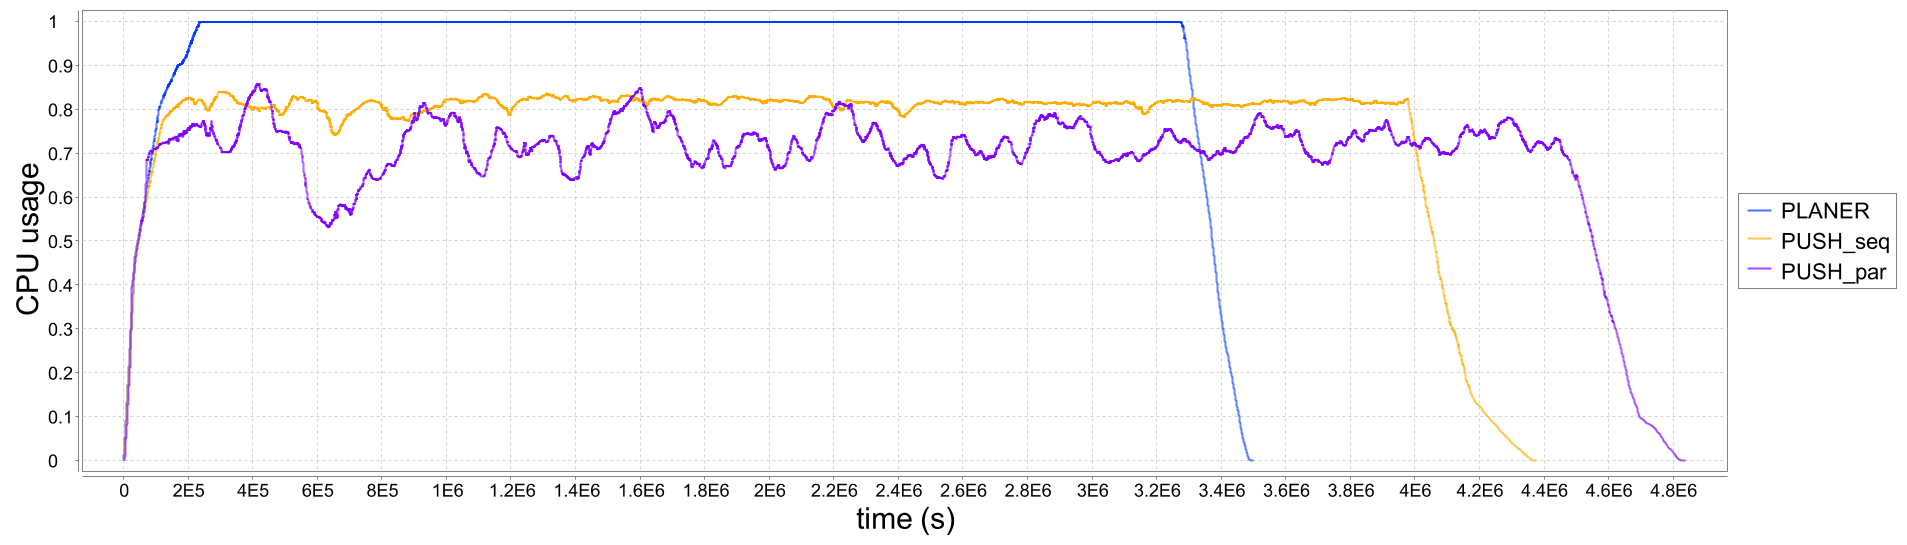
\includegraphics [trim= 0mm 00mm 0mm 00mm , clip,       	width=\textwidth]{pic/3models_link01.png}
    \caption{Comparison of CPU usage of three models. }
\end{figure}
\end{frame}


\begin{frame}\frametitle{Multiple nodes}
\begin{figure}[h]
\centering
\includegraphics [trim= 0mm 00mm 0mm 00mm , clip,       	width=\textwidth]{pic/3nodes_1storage_makespan_improvement.pdf}
    \caption{Makespan improvement of proposed model compared to PUSH par and PUSH seq}
\end{figure}
\end{frame}




\end{document}
